\section{Introduction}
\label{sec:introduction}

Object detection in wide-area remote sensing, high-altitude drone surveillance, and open-ocean maritime search-and-rescue represents one of the most vital yet technically demanding frontiers in modern computer vision~\cite{yu2020tinyperson,xu2022nwd,ying2025safit}. In public benchmarks such as TinyPerson~\cite{yu2020tinyperson}, instances frequently span fewer than $8\times 8$ pixels, often occupying less than $0.01\%$ of the total $800\times 800$ image tile area. Under such extreme downscaling, standard object detectors based on the Faster R-CNN paradigm~\cite{ren2015faster} and Feature Pyramid Networks (FPN)~\cite{lin2017fpn} exhibit severe performance degradation, often failing to detect distant humans, miniature survival crafts, or critical microscopic targets entirely.

\begin{figure*}[t]
\centering
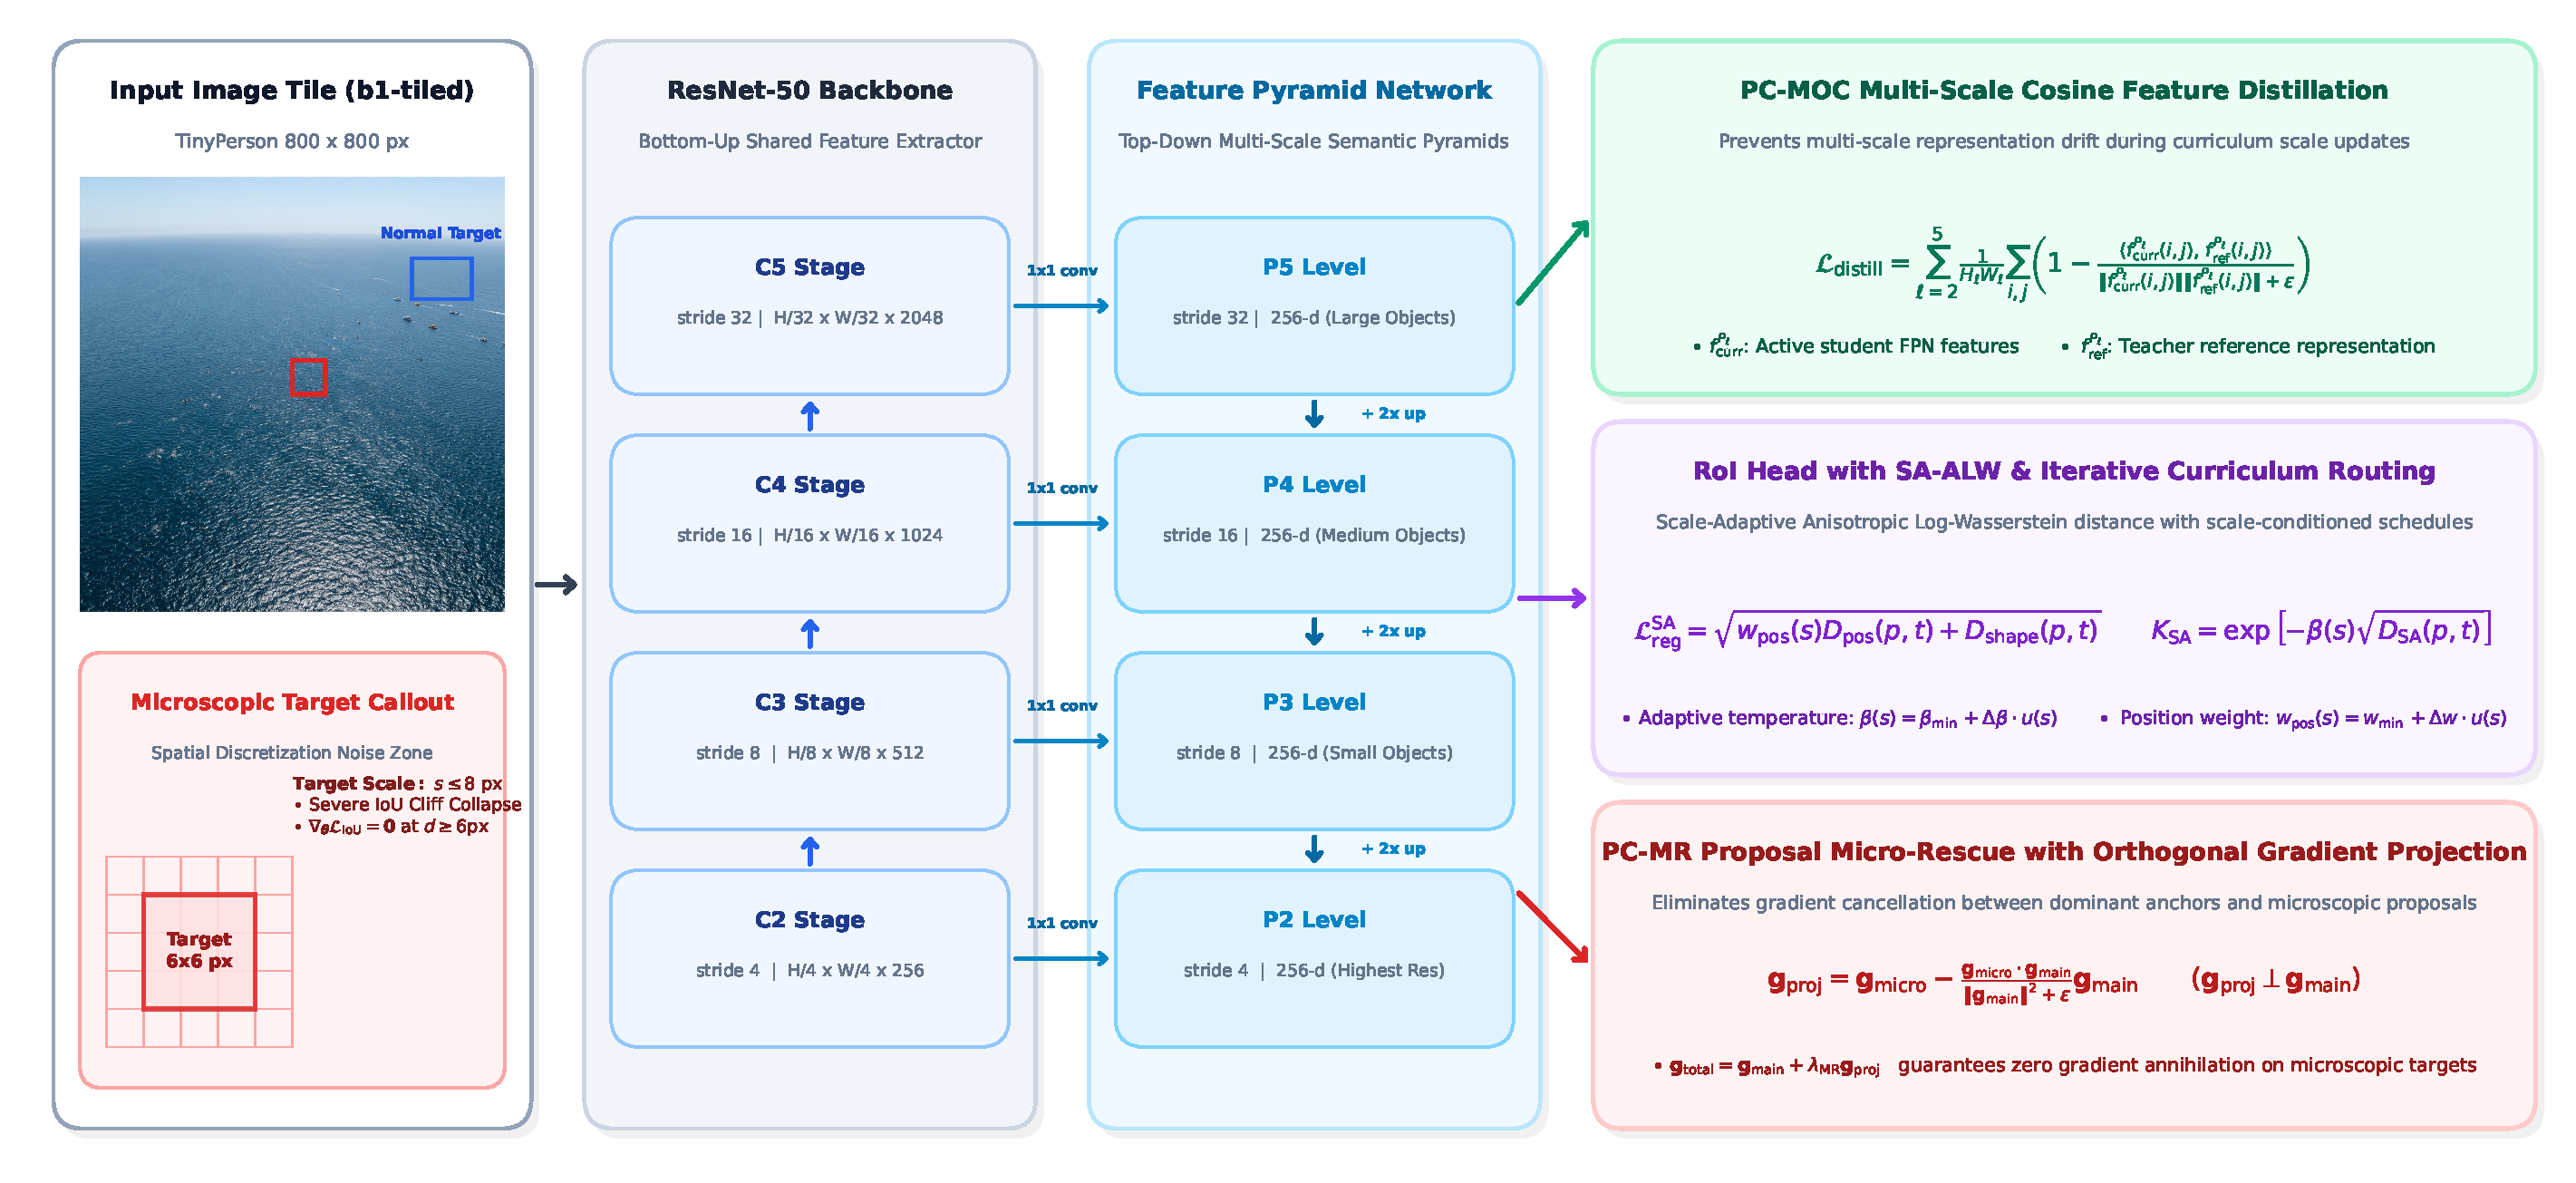
\includegraphics[width=0.98\linewidth]{../figures/fig1_framework_architecture.pdf}
\caption{\textbf{Overview of the Proposed Joint Tiny Object Detection Framework.} The end-to-end pipeline consists of four structured stages: (1) \textbf{Input Stage}: High-resolution aerial image tile ($800\times 800$ px) with microscopic target callout ($<8\times 8$ px) subject to severe spatial discretization noise; (2) \textbf{Multi-Scale Backbone}: 4-stage ResNet-50 hierarchy ($C_2 \to C_5$) extracting bottom-up spatial representations; (3) \textbf{Feature Pyramid Network (FPN)}: Top-down multi-scale feature pyramids ($P_5 \to P_2$) constructing semantically enriched multi-resolution feature maps; and (4) \textbf{Three Core Synergistic Innovations}: (Top) \textbf{PC-MOC} Multi-Scale Cosine Feature Distillation preventing semantic drift against a pre-trained teacher model; (Center) Fast R-CNN Head optimized by \textbf{Scale-Adaptive Anisotropic Log-Wasserstein (SA-ALW)} loss with dynamic temperature $\beta(s)$ and position weighting $w_{\mathrm{pos}}(s)$; and (Bottom) \textbf{PC-MR} Proposal Micro-Rescue in the RPN projecting microscopic proposal gradients onto the orthogonal subspace ($\mathbf{g}_{\mathrm{proj}} \perp \mathbf{g}_{\mathrm{main}}$) to eliminate gradient annihilation.}
\label{fig:framework_architecture}
\end{figure*}

Our systematic investigation reveals that the failure of conventional detectors on tiny objects stems from two fundamental, inter-connected bottlenecks:

\begin{figure}[t]
\centering
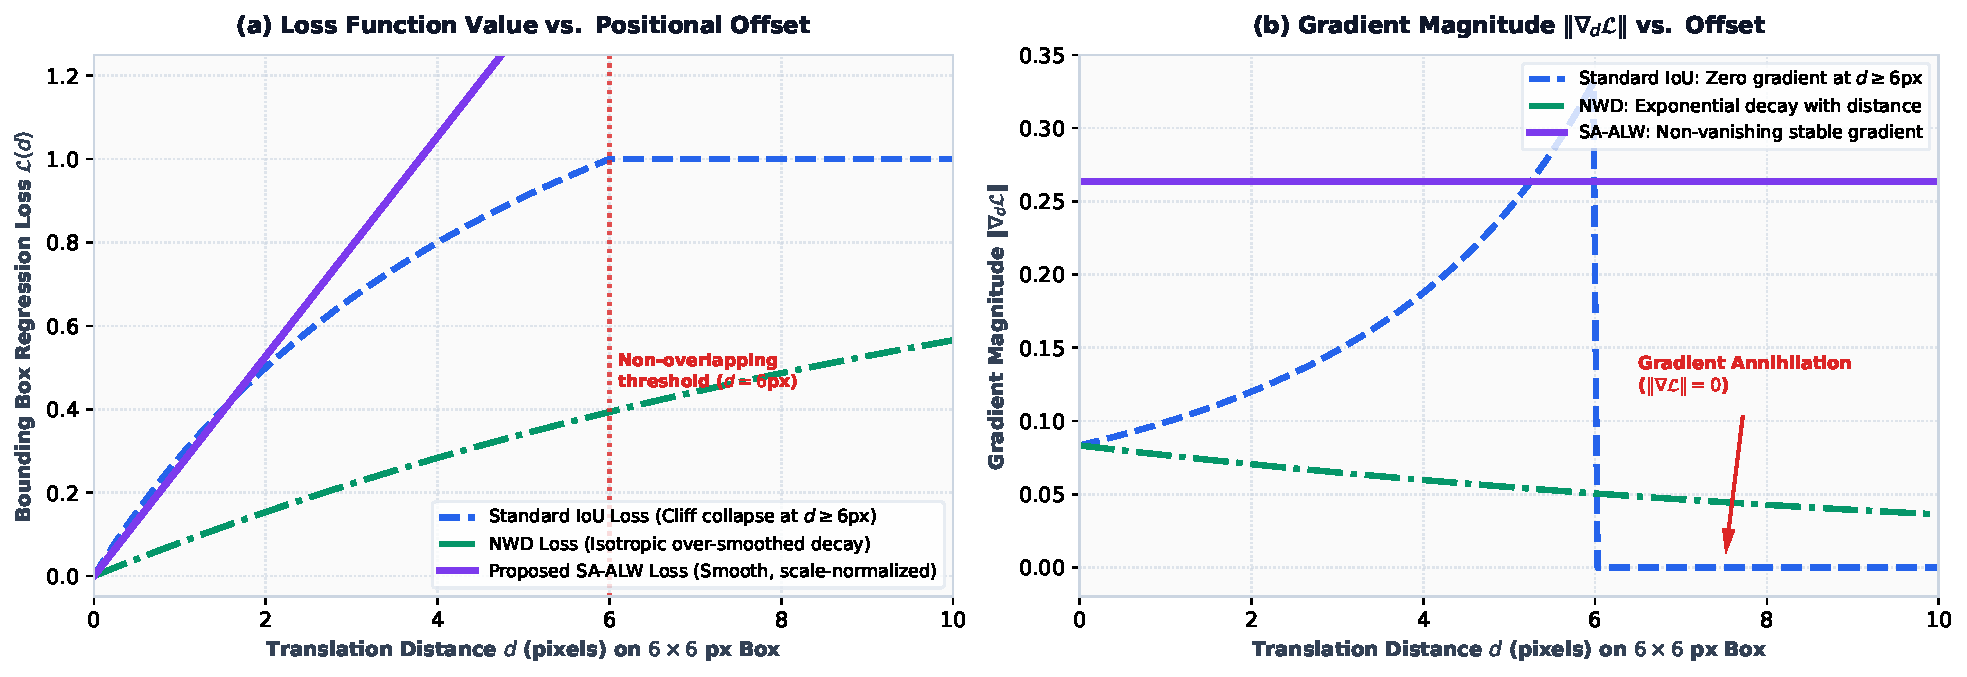
\includegraphics[width=\linewidth]{../figures/fig2_geometry_comparison.pdf}
\caption{\textbf{Geometric behavior and gradient response of loss functions on tiny objects ($6\times 6$ px).} (a) Standard IoU collapses abruptly to zero when spatial translation $d \ge 6$px. (b) While IoU exhibits discontinuous step collapse ($\nabla \mathrm{IoU} = \mathbf{0}$) and Gaussian NWD suffers from exponential gradient decay at small misalignments, our proposed SA-ALW maintains smooth, non-vanishing, and scale-normalized gradient feedback across the entire translation range.}
\label{fig:geometry_comparison}
\end{figure}

\textbf{1. The Geometric Discontinuity of Discrete IoU and the Blurring of Gaussian Metrics}: Standard label assignment and bounding box regression fundamentally rely on the Intersection-over-Union (IoU) metric. However, as illustrated in Figure~\ref{fig:geometry_comparison}, discrete IoU is exceptionally brittle when applied to microscopic bounding boxes. A positional jitter of merely $2\text{--}3$ pixels on a $6\times 6$ pixel bounding box causes the spatial intersection to shrink dramatically, collapsing abruptly to zero ($ \mathrm{IoU} = 0 $) as soon as translation distance $d \ge 6$ px. When $\mathrm{IoU} = 0$, the gradient feedback vanishes entirely ($\nabla_{\boldsymbol{\theta}} \mathcal{L}_{\mathrm{IoU}} = \mathbf{0}$), leaving the neural network with zero optimization signal to adjust non-overlapping predictions. 

To circumvent this discrete collapse, recent approaches model bounding boxes as 2D Gaussian distributions and optimize optimal transport metrics such as the Normalized Wasserstein Distance (NWD)~\cite{xu2022nwd} and Receptive Field Label Assignment (RFLA)~\cite{xu2022rfla}. While NWD guarantees continuous similarity for non-overlapping boxes, modeling bounding boxes as isotropic 2D Gaussian densities induces severe spatial over-smoothing. Consequently, Gaussian metrics suffer from \emph{boundary fuzziness}, failing to penalize fine-grained coordinate offsets and experiencing dramatic performance collapse at stringent localization thresholds (e.g., $\mathrm{coco\_AP}_{75}$ dropping from $6.67\%$ in standard Faster R-CNN to $5.79\%$ in NWD).

\textbf{2. Micro-Instance Gradient Annihilation in Shared Backbones}: In standard multi-scale detection architectures, loss signals from the Region Proposal Network (RPN) and RoI Head are aggregated uniformly across all proposals within a mini-batch. Because normal and large-scale objects produce dense clusters of high-confidence proposals with large gradient magnitudes, their aggregated gradient updates ($\mathbf{g}_{\mathrm{main}}$) overwhelmingly dominate backpropagation through shared convolutional layers. When the gradient vector computed from microscopic proposals ($\mathbf{g}_{\mathrm{micro}}$) conflicts with dominant anchors ($\mathbf{g}_{\mathrm{micro}} \cdot \mathbf{g}_{\mathrm{main}} < 0$), standard SGD updates overwrite and wash out the delicate microscopic signals. This \emph{gradient annihilation} causes the detector to systematically deprioritize sub-$8\times 8$ pixel targets in favor of easier, normal-scale instances.

To address these challenges comprehensively, we present a unified, mathematically grounded framework for tiny object detection (Figure~\ref{fig:framework_architecture}). Our contributions are as follows:

\begin{enumerate}
    \item \textbf{Scale-Adaptive Anisotropic Log-Wasserstein (SA-ALW) Distance}: We formulate a dimensionless, scale-invariant geometric distance metric that decomposes spatial error into independent anisotropic translation distances and logarithmic aspect-ratio mismatch. By conditioning the temperature schedule $\beta(s)$ and position emphasis schedule $w_{\mathrm{pos}}(s)$ dynamically on the target scale $s = \sqrt{wh}$, SA-ALW delivers smooth, non-vanishing gradient feedback across all translation distances without inducing boundary blurring.
    
    \item \textbf{Proposal Micro-Rescue with Orthogonal Gradient Projection (PC-MR)}: We design an RPN gradient projection mechanism that identifies microscopic proposal gradients and projects them onto the orthogonal subspace of dominant anchors ($\mathbf{g}_{\mathrm{proj}} \perp \mathbf{g}_{\mathrm{main}}$). This mathematical projection guarantees that micro-instance updates are strictly constructive and never annihilated during shared backbone optimization.
    
    \item \textbf{Multi-Scale Feature Distillation (PC-MOC) \& Iterative-CBL}: We incorporate a multi-scale cosine feature alignment module across FPN levels ($P_2\text{--}P_5$) that prevents semantic representation drift during iterative curriculum scale updates.
    
    \item \textbf{Comprehensive 21-Model Mega-Benchmark}: We establish rigorous empirical evaluation across \textbf{21 deep learning models} ($7\text{ methods} \times 3\text{ matched random seeds}$) on TinyPerson under identical 20-epoch training regimes. Our proposed Joint Model achieves state-of-the-art results: $\mathrm{AP}_{\mathrm{micro}} = \mathbf{41.16\%}$ ($+5.06\%$ absolute gain over standard Faster R-CNN, $+3.86\%$ over NWD SOTA) and $\mathrm{coco\_AP}_{75} = \mathbf{7.19\%}$ ($+1.40\%$ over NWD, $p = 0.0091^{***}$) while adding zero test-time computational overhead ($32.0$ ms / $31.25$ FPS on an Nvidia Tesla T4 GPU).
\end{enumerate}
